%--------------------------------------
% Create title frame
\titleframe

%--------------------------------------
% Table of contents
\begin{frame}{Overview}
  \setbeamertemplate{section in toc}[sections numbered]
  \tableofcontents[hideallsubsections]
\end{frame}


%==============================================
%\section{Overview}
\subsection{iHub-Data}
\begin{frame}{\insertsubsectionhead}
  \framesubtitle{Overview}
  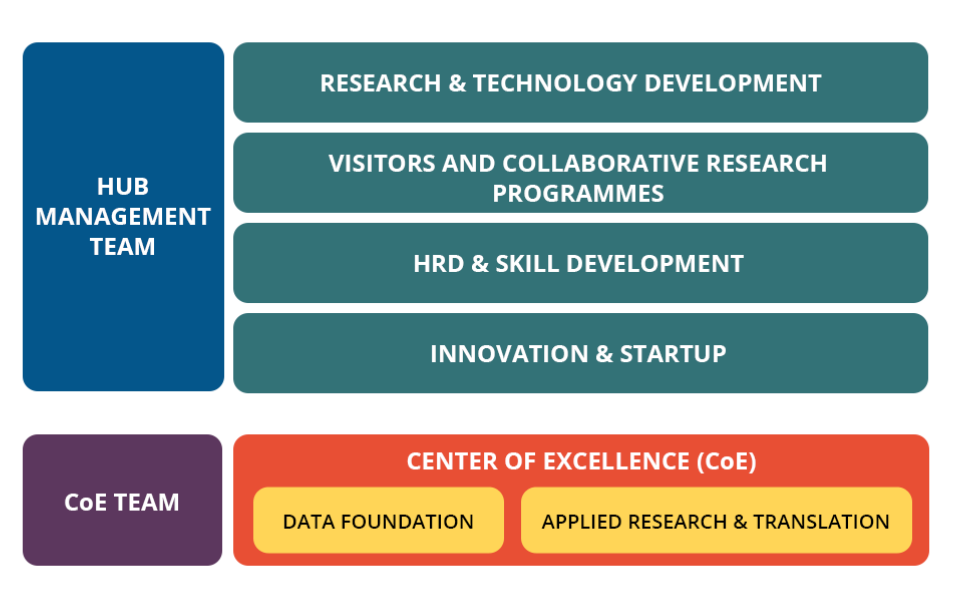
\includegraphics[scale=0.3]{images/overview.png}
\end{frame}

\subsection{Programs}
\begin{frame}{\insertsubsectionhead}
  \framesubtitle{Verticals}
  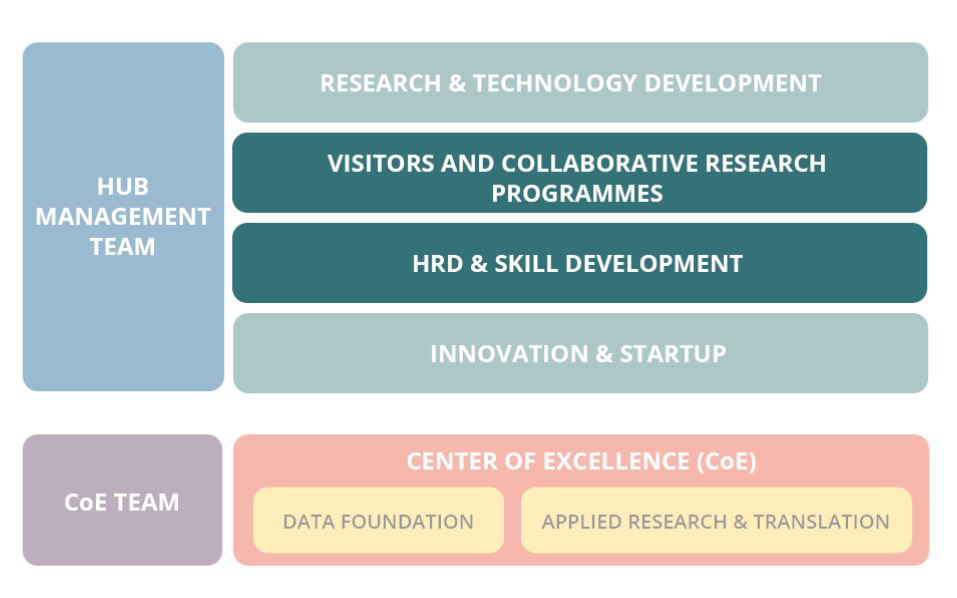
\includegraphics[scale=0.3]{images/overview-1.png}
\end{frame}
%==============================================
\section{\textbf{HRD}}

\begin{frame}[fragile=singleslide]{}
\begin{center}
\begin {itemize}
\item {\textbf{UG Research Programs}} - Strengthen existing UG research - support conferences/internships of internal students
\item {Masters Fellowships} - Support graduate students working in data-driven technologies to take up well-planned research activities
\item {PhD Fellowships} - Support PhD fellowships in data-driven technologies in areas of Hub
\item {\textbf{PostDoc Fellowships}} - Support postdoc fellowships to work with senior members of Hub/Institute for relevant technology development in areas of Hub
\item {\textbf{Tenure Track Faculty Fellowship}} - To help independent motivated researchers jump start their career through proper guidance and support in areas of Hub
\item {\textbf{Chair Professorship}} - To enable senior faculty members to dedicate more time/effort to provide direction and guidance to  young researchers in areas of Hub
\item {\textbf{Summer/Winter Schools}} - Extend such programs to widen audience - students/teachers/researchers/working professionals - conducted by Hub
\end{itemize}
\end{center}
\end{frame}



\begin{frame}[fragile=singleslide]{}
\begin{center}
\begin {itemize}
%\item Mini Symposium Over \textbf{29 July 2022}
%\item 10 participants 
\item Ms Dharani informed to claim 595 euro fees, after submitting bills (scholar of Prof Vishal Garg)
\item Two MS Fellowship applicants in their final year of MSc (Bioinformatics) and M Tech (Agri Tech)
\item Ms Stuti - Inspire-DST cleared scholar - Bioinformatics - PhD Supervisor  (received on Monday)
\item Write-up for Tenure Track - Chair Professor/Faculty Fellows (not yet)
\item Winter Project Internship  - Translation - Final decision awaited
\end{itemize}
\end{center}
\end{frame}

\section{Skill Development }
\begin{frame}[fragile=singleslide]{\insertsectionhead}
  \framesubtitle{\insertsubsectionhead}
\begin{center}
\begin{itemize}
\item Foundations of Modern Machine Learning - (2021-22) 129 passed
%\item Foundations of Modern Machine Learning - (2022) 43 passed
%\item Machine Learning for Chemistry and Drug Discovery (2022) 167 passed
\item Financial Rewards to Winners were announced in the beginning 
\begin{itemize}
\item Top 5 percent of qualifiers would get Rs 25K
\item Three candidates
\item Next 10 percent would get Rs 15K
\item Six candidates
\item Additional Prize Money - Rs 93k (Rs 8k has been already refunded to all qualified candidates)
\end{itemize}
\item Video feedback from participants have been archived
\end{itemize}
\end{center}
\end{frame}

\subsection{Online Programs}
\begin{frame}[fragile=singleslide]{\insertsectionhead}
  \framesubtitle{\insertsubsectionhead}
  \textbf  Off-campus Programs
  \begin{itemize}
    \item Foundations of Modern Machine Learning - 2022 (commenced)
   \item Bridge sessions in progress for All India Students
    \item 473 students - All-India-Students (122) + Raj-Reddy-Centre (351) 
    \item Rural students to join later this month (Aug)
\item Main sessions to commence by end September
    \item 9 existing TAs + 5 new 
    \item TAship compensation - Revised for institute
  \end{itemize}
\end{frame}



\subsection{On-Campus Programs}
\begin{frame}[fragile=singleslide]{\insertsectionhead}
  \framesubtitle{\insertsubsectionhead}
  \textbf  On-campus Programs
  \begin{itemize}
    \item DRDO - Quarterly Program - in advanced stage
    \item Advanced Machine Learning Program - in planning stage
    \item  Long term - create translation engineers with inhouse training (?)
  \end{itemize}
\end{frame}

%==============================================
\section{Visitors}
%==============================================

\subsection{Categories of Visitors}
\begin{frame}[fragile=singleslide]{\insertsectionhead}
  \framesubtitle{\insertsubsectionhead}
\begin{center}
\begin{itemize}
%\item 126 Summer School Internships (over)
%\item 30 Faculty Resource Persons of CVIT Summer School (ongoing)
\item 1 Visiting Faculty (short term Dr Hafez) - Project under Mobility (ongoing)
\item First instalment of Rs 25k towards accommodation, food for 10 days
%\item SRISHTI -Gift Coupons distributed
\item Summer School - Gift/Remuneration after Aug/19
\item Token share income from CVIT - to be taken up after Aug/19
\end{itemize}
\end{center}
\end{frame}


%==============================================
%\section{8-week Summer Research Internship}
%==============================================





%==============================================
\section{Collaborative Research Programs}
%==============================================

\subsection{Program Details}
\begin{frame}[fragile=singleslide]{\insertsectionhead}
  \frametitle {8 Regions in India - Commenced}
\begin{center}
\begin{itemize}
%\item Short-term Training Programs in AI/ML (5 institutions per region)
%\item Support for Conferences in AI/ML (5 institutions per region)
%\item Support for Student/Faculty Development Workshops in AI/ML (5 institutions per region)
\item Two conferences - Our committee can select best paper and decide on award
\item Committee Members - Maitreya Maity..
\item Present Hub's view in advance and during award ceremony
\end{itemize}
\end{center}
\end{frame}


\subsection{National Expo}
\begin{frame}[fragile=singleslide]{\insertsubsectionhead}
  \frametitle {National Expo - Mobility/Healthcare/Data Foundation}
\begin{center}
\begin{itemize}
\item Advt about to be released
\item Delayed - previous payment issue
\item Whether Pavan can be tested here ?
%\item Healthcare - in progress 
%\item Other Streams - in progress
%\item One HPC Workshop by CDAC
\item Venue - T-Hub ?
\end{itemize}
\end{center}
\end{frame}


\subsection{National Expo}
\begin{frame}[fragile=singleslide]{\insertsubsectionhead}
  \frametitle {National Expo - Themes}
\begin{center}
\begin{itemize}
   \item CEO/CTO Speak – Successes and Challenges
    \item AI/ML Deep-Tech Project Landscape
    \item Training Programs on AI/ML
    \item C-DAC Workshop on HPC
    \item Start-ups – Stories on AI/ML
    \item PSUs/NGOs – AI/ML Services
\end{itemize}
\end{center}
\end{frame}
%
%%==============================================
%\section{Ongoing Programs}
%%==============================================
%
%\subsection{Ongoing}
%
%\begin{frame}[fragile=singleslide]{\insertsectionhead}
% % \framesubtitle{\insertsubsectionhead}
%\begin{center}
%\begin{itemize}
%\item 50-week FMML commencing from August 2022
%\item SRISHTI - 22
%\item National Expo Data-Driven Solutions NEDDS-22
%\begin{itemize}
%\item Stakeholders from NM-ICPS - Govt, Academics, Industry, Start-ups, NGOs
%\end{itemize}
%\item Springer LNCS International Conference on BDA2022 (Big Data Analytics) 
%\begin{itemize}
%\item Co-organiser
%\end{itemize}
%\end{itemize}
%\end{center}
%\end{frame}
%
%\subsection{\\50-week FMML - Aug 22}
%
%\begin{frame}[fragile=singleslide]{\insertsectionhead - \insertsubsectionhead}
% % \framesubtitle{\insertsubsectionhead}
%\begin{center}
%\begin{itemize}
%\item Based on learnings from prior FMML programs
%\item Entry based on aptitude scores
%\item Academic inclination - more homogeneous
%\item Target - second year UG students only
%\item Administer course modulewise -  one teacher per module
%\item Hire permanent teachers/mentors - underway
%\item DST confidence-building measure (large figures)
%\end{itemize}
%\end{center}
%\end{frame}
%
%
%\subsection{Program Details}
%\begin{frame}[fragile=singleslide]{\insertsectionhead}
%  \framesubtitle{\insertsubsectionhead}
%\begin{center}
%\begin{itemize}
%\item Summer Internship Program at IIIT Hyderabad
%\item \textbf{Period : } 16 May to 30 Jun
%\item iHub funded Internship Program Rs 10,000 per student
%\item Preliminary Selection from 7600+ (2650) students all over India
%\item Admission Procedure - Exam (online + offline)
%\item 126 students to work in thirteen Research Centres
%\item 23 members of faculty currently supervising interns
%\item Centralised training program (TNA) progressing simultaneously
%\item 90 students listed to work remotely (unpaid)
%\item \textbf{Waiting List : } Another 450 candidates, shared internally
%\end{itemize}
%\end{center}
%\end{frame}
%
%
%\subsection{\\SRISHTI 22}
%
%\begin{frame}[fragile=singleslide]{\insertsectionhead - \insertsubsectionhead}
% % \framesubtitle{\insertsubsectionhead}
%\begin{center}
%\begin{itemize}
%\item Goals, Objectives
%\begin{itemize}
%\item To imbibe a sense of academic and research inquiry to interns
%\end{itemize}
%\item Set expectations of interns
%\begin{itemize}
%\item Cognitive, General Skills, Personal 
%\end{itemize}
%\item Resources to interns
%\begin{itemize}
%\item Infrastructure, Compute
%\end{itemize}
%\item Success Metrics
%\begin{itemize}
%\item 40 percent of supervisors will re-appear next year
%\item 20 percent of interns would publish a paper in a year
%\item 10 percent of interns contribution would lead to product/patent in a year
%\item 80 percent interns would report high satisfaction
%\end{itemize}
%\end{itemize}
%\end{center}
%\end{frame}
%
%\subsection{\\SRISHTI 22}
%
%\begin{frame}[fragile=singleslide]{\insertsectionhead - \insertsubsectionhead}
% % \framesubtitle{\insertsubsectionhead}
%\begin{center}
%\begin{itemize}
%\item 11:30 am - 2:30 pm - Lectures/Tutorials/Special Sessions (all weekdays from 18 May to 24 June)
%\item Progress Monitoring on Wednesdays - 18 May, 25  May, 01 June, 08 June, 15 June, 22 June	 
%\end{itemize}
%\end{center}
%\end{frame}
%
%\subsection{\\National-level Expo in November}
%
%\begin{frame}[fragile=singleslide]{\insertsectionhead - \insertsubsectionhead}
% % \framesubtitle{\insertsubsectionhead}
%\begin{center}
%\begin{itemize}
%\item C-DAC India agrees to be a partner 
%\item Workshop on HPC on second day
%\item Exploring options with Intel India
%\end{itemize}
%\end{center}
%\end{frame}
%
%%==============================================
%\section{Fresh Plans}
%%==============================================
%
%\subsection{Outreach Activities}
%
%\begin{frame}[fragile=singleslide]{\insertsectionhead}
%  \framesubtitle{\insertsubsectionhead}
%\begin{center}
%\begin{itemize}
%\item Scale Online Courses - Public Universities
%\item Explore Long-term Online Internships - about to commence
%\item Approach NIELIT for exploring joint online program
%\item Joint Workshop bda2022.org Dec 19-22, 2022 at Hyderabad
%\end{itemize}
%\end{center}
%\end{frame}
%
%

%-------------------------------------
%\end{document}
%--------------------------------------
